% This is samplepaper.tex, a sample chapter demonstrating the
% LLNCS macro package for Springer Computer Science proceedings;
% Version 2.20 of 2017/10/04
%
\documentclass[runningheads]{llncs}
%
\usepackage{graphicx}
\usepackage{float}
\usepackage{subcaption}
\usepackage{dirtytalk}
\captionsetup{compatibility=false}



% Used for displaying a sample figure. If possible, figure files should
% be included in EPS format.
%
% If you use the hyperref package, please uncomment the following line
% to display URLs in blue roman font according to Springer's eBook style:
% \renewcommand\UrlFont{\color{blue}\rmfamily}

\begin{document}
%
\title{Bachelor Dissertation}
%
%\titlerunning{Abbreviated paper title}
% If the paper title is too long for the running head, you can set
% an abbreviated paper title here
%
\author{Kasper Engelen\and
		Jonathan Meyer\and
		Dawid Miroyan\and
		Igor Schittekat}
%
%
\institute{University of Antwerp}
%
\maketitle              % typeset the header of the contribution
%
\begin{abstract}
This document reports our findings regarding the final dissertation. The sections and subsections correspond to the assignments given to us. In this project we worked with a simulator called Stride, developed at the University of Antwerp. We explore various concepts within computational epidemiology through the use of this program. 

\keywords{Computational Epidemiology  \and Dissertation}
\end{abstract}
%
%
%

\section{Introduction}


\section{Daycare \& PreSchool}
\paragraph{}
The first feature is the addition of two new ContactTypes, namely the Daycare and PreSchool. Here children from ages 0 to 3 can participate in a Daycare, whereas children from ages 3 to 6 can go to a PreSchool. Both ContactTypes make use of a participation parameter to determine how many of these children actually will go to these ContactTypes.


\section{Demographic profile}

\section{Workplace Size Distribution}
\paragraph{}
With the addition of the third feature, we can specify different ranges of sizes for workplaces. This means we can have 70\% of workplaces that have a size between 20 and 50 and 30\% between 50 and 100.

The workplace size distribution used in the new algorithm as the default case is the following:
\begin{table}[!h]
	\centering
	\begin{tabular}{|c|c|c|}
		\hline
		Ratio & Minimum size & Maximum size \\\hline
		77.854\% & 1 & 9 \\\hline
		17.190\% & 10 & 49 \\\hline
		4.100\% & 50 & 199 \\\hline
		0.856\% & 200 & 400 \\\hline
	\end{tabular}
\end{table}

while in the original algorithm, all the workplaces are around 20 people large.

To determine whether different size classes in the workplaces have a significant impact on the simulations, the influenza virus is used.
Here, more interesting results, meaning there is a noticeable difference in simulation results, can be seen when the immunity rate is sufficiently low. For this reason we used an immunity rate of 40\%, this means that 60\% of the population can get infected by the influenza virus.
The new algorithm is compared to different sizes of workplaces using the different algorithm, with size 17 being the average for the values used in the new algorithm.

\begin{figure}[h!]
	\centering
	\begin{subfigure}[b]{0.6\linewidth}
		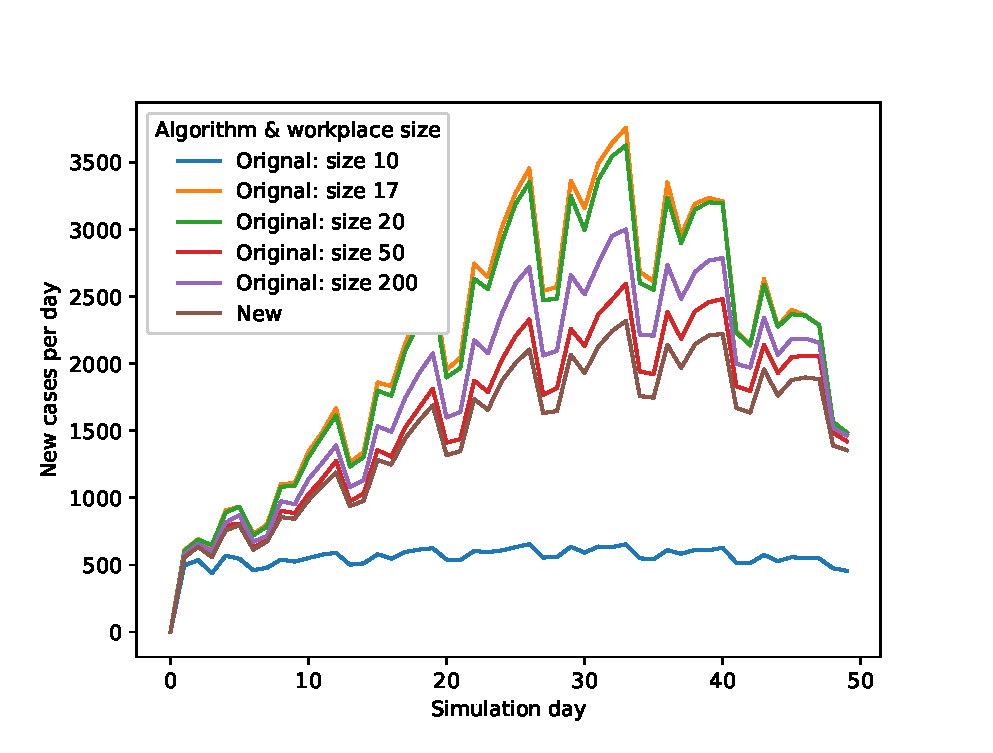
\includegraphics[width=\linewidth]{Workplace/workplace_sizes_ncpd.eps}
		\caption{Average new cases per day.}
	\end{subfigure}
	\begin{subfigure}[b]{0.6\linewidth}
		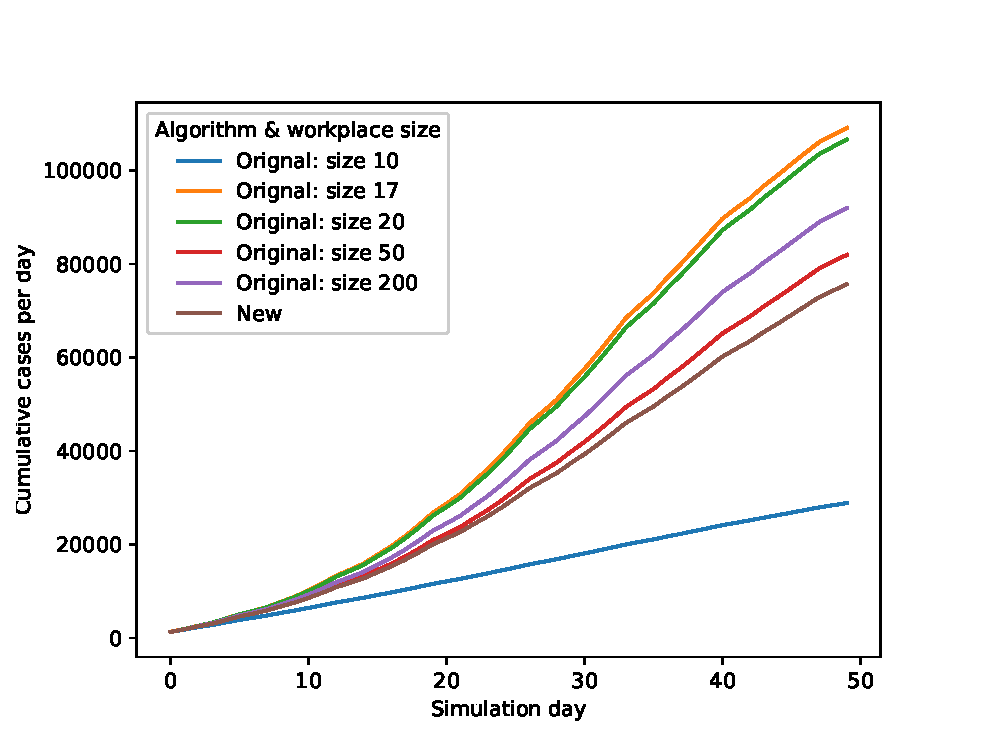
\includegraphics[width=\linewidth]{Workplace/workplace_sizes_ccpd.eps}
		\caption{Average cumulative cases.}
	\end{subfigure}
	\caption{Results of 20 different simulations for varying workplace sizes. Seeding rate = $0.2\%$, immunity rate = $40\%$, $R_0$ = 2. Simulated for a population of 600,000 over 50 days.}
	\label{workplace_immunity}
\end{figure}

The most noticeable result is how a decreasing workplace size leads to more new cases per day, this happens until around size 10 where the amount of new cases drops significantly. Very small workplaces do not allow the disease to spread quickly when compared to the larger ones. A possible explanation here is that the chance to meet an infected person in these workplaces is small.

The average size of workplaces in the new algorithm does not seem to be an important factor.

While running a simulation using the original algorithm and having results of the new algorithm seems possible, finding the correct size of the workplaces is difficult. Each different size of the workplace has their own impact on the spread of the disease, so we can conclude that a combination of those sizes result in a more realistic spread.

\end{document}
